\documentclass[journal]{IEEEtran}

%\usepackage{polski}
\usepackage[T1]{fontenc}
\usepackage[utf8]{inputenc}
\usepackage[pdftex]{graphicx}
\graphicspath{{img/}}

% correct bad hyphenation here
\hyphenation{naj-waż-niej-sze neu-ro-no-we}


\begin{document}
%
% paper title
% can use linebreaks \\ within to get better formatting as desired
\title{Rozpoznawanie języka tekstu \\ na podstawie częstotliwości liter}

\author{Krzysztof~Kutt, Michał~Nowak
\thanks{K. Kutt i M. Nowak, Katedra Automatyki, Wydział Elektrotechniki, Automatyki, Informatyki i Elektroniki,
Akademia Górniczo-Hutnicza, Kraków, Polska, e-mail: kkutt@student.agh.edu.pl, rial@student.agh.edu.pl}}

\markboth{Sztuczne Sieci Neuronowe, semestr letni 2011/2012, prowadzący: mgr inż. Tomasz Orzechowski}%
{}

% make the title area
\maketitle


\begin{abstract}
W artykule przedstawiono problem rozpoznawania języka zadanego tekstu i propozycje jego rozwiązania.
Autorzy zdecydowali się na wykorzystanie informacji o częstotliwości występowania liter. Przygotowano
program wykorzystujący sieć neuronową i zestaw danych uczących. W trakcie testów osiągnięto dobrą skuteczność.
Zaproponowano możliwości dalszego rozwoju projektu.
\end{abstract}

% Note that keywords are not normally used for peerreview papers.
\begin{IEEEkeywords}
sieć neuronowa, język naturalny, częstotliwość liter.
\end{IEEEkeywords}


\section{Wprowadzenie}
% The very first letter is a 2 line initial drop letter followed
% by the rest of the first word in caps.
% 
% form to use if the first word consists of a single letter:
% \IEEEPARstart{A}{demo} file is ....
% 
% form to use if you need the single drop letter followed by
% normal text (unknown if ever used by IEEE):
% \IEEEPARstart{A}{}demo file is ....
% 
% Some journals put the first two words in caps:
% \IEEEPARstart{T}{his demo} file is ....
% 
% Here we have the typical use of a "T" for an initial drop letter
% and "HIS" in caps to complete the first word.
%
% You must have at least 2 lines in the paragraph with the drop letter
% (should never be an issue)

\IEEEPARstart{S}{ztuczne} sieci neuronowe to bardzo uproszczone modele ludzkiego mózgu.
Każda z sieci składa się z setek, albo tysięcy sztucznych neuronów, stworzonych na wzór naturalnego
neuronu. Sztuczny neuron zbiera sygnały wejścia (poprzez 'dendryty'), dokonuje na nich odpowiedniej
transformacji i zwraca odpowiednią wartość na wyjściu ('akson'). W zależności od budowy sieci (układu
neuronów) oraz od wykorzystywanej przez neurony funkcji aktywacji, wyróżniane są różne rodzaje sieci~\cite{tad:sieci}.

\subsection{Rodzaje sieci}
Najważniejsze typy sieci neuronowych to sieci jednokierunkowe, sieci rekurencyjne i~sieci Kohonena~\cite{wiki:sieci}.

\subsubsection{Sieci jednokierunkowe}
W tych sieciach neurony są ułożone warstwowo. Sygnały przechodzą od wejścia do wyjścia sieci, przez wszystkie jej
warstwy, bez nawrotów (bez sprzężenia zwrotnego). Rozwiązują dosyć szeroką klasę problemów.

\subsubsection{Sieci rekurencyjne}
Sieci ze sprzężeniem zwrotnym. Połączenia między neuronami stanowią graf z cyklami. Stosowane są np do rozwiązywania
problemów minimalizacji, przykładowo: problemu komiwojażera.

\subsubsection{Sieci Kohonena}
Sieć, która dopasowuje swoją strukturę przestrzenną do zbioru danych (mapa). Uczona bez nauczyciela.


\subsection{Zastosowania sieci}
Sztuczne sieci neuronowe, ze względu na fakt podawania jedynie przybliżonych wyników, nie nadają się do obliczania
dokładnych wartości. Za to, dzięki 'umiejętności' uczenia się, nadają się do rozwiązywania problemów słabo określonych,
do których nie jesteśmy w stanie stworzyć algorytmów. Sieć w trakcie procesu uczenia się może wykryć zależności,
których nie jesteśmy w stanie dostrzec.

Przykładowymi problemami, do których sieci neuronowe są odpowiednimi
narzędziami, są: rozpoznawanie pisma, przetwarzanie obrazu (np w poszukiwaniu ukrtych jednostek wojskowych, czy
podejrzanych pakunków na lotniskach), prognozowanie cen.


\subsection{Rozpoznawanie języka zadanego tekstu}
W niniejszym artykule przedstawiony zostaje inny, ciekawy problem: rozpoznawanie języka zadanego tekstu.

Wg projektu ``Ethnologue'', na świecie istnieje prawie 7.5 tysiąca języków~\cite{ethnologue}. Narzędzie,
które byłoby w stanie rozpoznać z jakim językiem mamy doczynienia, byłoby bardzo użyteczne - dzięki niemu,
można np ustalić jakiego tłumacza potrzebujemy. Wizją przyszłości jest stworzenie automatycznego tłumacza,
który najpierw rozpoznaje mowę naszego rozmówcy, następnie rozpoznaje język, tłumaczy go, a na samym końcu
syntezuje mowę, byśmy mogli w naszym ojczystym języku usłyszeć słowa rozmówcy.

Do zadania tego można podejść na wiele sposobów~\cite{smykowski:jak_google_rozpoznaje}.

\subsubsection{Alfabet}
Pierwszą przesłanką może być wykorzystywany alfabet. Wiele języków posiada charakterystyczne dla siebie znaki
diakrytyczne, jak np język polski i 'ogonki'.

\subsubsection{Charakterystyczne wyrazy}
W przypadku takich samych alfabetów, decyzję o języku można podjąć, zwracając uwagę na charakterystyczne dla
danego języka wyrazy, czy końcówki. Duże zestawienie takich prostych reguł znajduje się w serwisie Wikipedia~\cite{wiki:langs}.

\subsubsection{Częstotliwość liter}
Można również ustalić częstotliwość występowania poszczególnych liter. Już krótkie spojrzenie na listę zestawów do gry
w Scrabble w różnych językach~\cite{wiki:scrabble} (ilość i wartość danej litery zależy od częstotliwości jej występowania
w danym języku), pozwala na stwierdzenie, że częstotliwości te są różne w różnych językach. Nie jest jednak możliwe proste
określenie reguł rozpoznawania języka na tej podstawie. Dlatego idealnym narzędziem do operowania na takich danych jest
sieć neuronowa.


\subsection{Rozpoznawanie języka na podstawie częstotliwości liter}
Niniejszy artykuł przedstawia próbę rozpoznawania języka na podstawie częstotliwości liter. Celem uproszczenia budowy
programu, zrezygnowano z analizy alfabetu i zdecydowano się na analizowanie tylko i wyłącznie częstotliwości 26~liter
alfabetu łacińskiego.

\subsubsection{Liczba wejść i wyjść}
Sieć składa się z 26 wejść: na każdym podawana jest częstotliwość występowania odpowiedniej litery alfabetu łacińskiego
w danym tekście. Liczba wyjść zależna jest od założonej ilości rozpoznawanych języków. W~przygotowanej aplikacji założono
obsługę 11 języków.

\subsubsection{Budowa sieci}
Ze względu na charakter zadania, czyli potrzebę wykrycia odpowiednich zależności w zestawie 26~sygnałów wejściowych,
zdecydowano się na wykorzystanie sieci jednokierunkowej, złożonej z trzech warstw (dodatkowa warstwa celem usprawnienia
procesu uczenia sieci). Nie istnieje żaden algorytm wspomagający podejmowanie decyzji o ilości neuronów w warstwie
ukrytej~\cite{tad:elem_wpr}. Decyzja ta jest zawsze podejmowana arbitralnie i następnie weryfikowana w czasie testów.
Należy tylko pamiętać, aby nie była ani zbyt duża, ani zbyt mała. Zdecydowano się przyjąć, że będzie się ona składała
z 10 neuronów.

\subsubsection{Funkcja aktywacji}
Każdy neuron wykorzystuje sigmoidalną funkcję aktywacji. Pozwala ona na lepsze różnicowanie zbliżonych sygnałów niż funkcja
liniowa. W rozważanym problemie, pozwala na lepsze różnicowanie zbliżonych częstotliwości występowania liter.

\subsubsection{Uczenie sieci}
Do uczenia sieci wykorzystano algorytm Resilient Propagation. Jest to zmodyfikowana wersja podstawowego algorytmu uczenia
z nauczycielem sieci wielowarstwowych jednokierunkowych, czyli algorytmu propagacji wstecznej. Zdecydowano się na ten
algorytm, ponieważ jest on najbardziej efektywnym algorytmem uczenia dla prostych sieci neuronowych, takich jak nasza~\cite{encog:rprop}.



% An example of a floating figure using the graphicx package.
% Note that \label must occur AFTER (or within) \caption.
% For figures, \caption should occur after the \includegraphics.
% Note that IEEEtran v1.7 and later has special internal code that
% is designed to preserve the operation of \label within \caption
% even when the captionsoff option is in effect. However, because
% of issues like this, it may be the safest practice to put all your
% \label just after \caption rather than within \caption{}.
%
% Reminder: the "draftcls" or "draftclsnofoot", not "draft", class
% option should be used if it is desired that the figures are to be
% displayed while in draft mode.
%
%\begin{figure}[!t]
%\centering
%\includegraphics[width=2.5in]{myfigure}
% where an .eps filename suffix will be assumed under latex, 
% and a .pdf suffix will be assumed for pdflatex; or what has been declared
% via \DeclareGraphicsExtensions.
%\caption{Simulation Results}
%\label{fig_sim}
%\end{figure}

% Note that IEEE typically puts floats only at the top, even when this
% results in a large percentage of a column being occupied by floats.


% An example of a double column floating figure using two subfigures.
% (The subfig.sty package must be loaded for this to work.)
% The subfigure \label commands are set within each subfloat command, the
% \label for the overall figure must come after \caption.
% \hfil must be used as a separator to get equal spacing.
% The subfigure.sty package works much the same way, except \subfigure is
% used instead of \subfloat.
%
%\begin{figure*}[!t]
%\centerline{\subfloat[Case I]\includegraphics[width=2.5in]{subfigcase1}%
%\label{fig_first_case}}
%\hfil
%\subfloat[Case II]{\includegraphics[width=2.5in]{subfigcase2}%
%\label{fig_second_case}}}
%\caption{Simulation results}
%\label{fig_sim}
%\end{figure*}
%
% Note that often IEEE papers with subfigures do not employ subfigure
% captions (using the optional argument to \subfloat), but instead will
% reference/describe all of them (a), (b), etc., within the main caption.


% An example of a floating table. Note that, for IEEE style tables, the 
% \caption command should come BEFORE the table. Table text will default to
% \footnotesize as IEEE normally uses this smaller font for tables.
% The \label must come after \caption as always.
%
%\begin{table}[!t]
%% increase table row spacing, adjust to taste
%\renewcommand{\arraystretch}{1.3}
% if using array.sty, it might be a good idea to tweak the value of
% \extrarowheight as needed to properly center the text within the cells
%\caption{An Example of a Table}
%\label{table_example}
%\centering
%% Some packages, such as MDW tools, offer better commands for making tables
%% than the plain LaTeX2e tabular which is used here.
%\begin{tabular}{|c||c|}
%\hline
%One & Two\\
%\hline
%Three & Four\\
%\hline
%\end{tabular}
%\end{table}


% Note that IEEE does not put floats in the very first column - or typically
% anywhere on the first page for that matter. Also, in-text middle ("here")
% positioning is not used. Most IEEE journals use top floats exclusively.
% Note that, LaTeX2e, unlike IEEE journals, places footnotes above bottom
% floats. This can be corrected via the \fnbelowfloat command of the
% stfloats package.

\section{Specyfikacja wymagań}
\IEEEPARstart{P}{odczas} analizy problemu zidentyfikowano dwa najważniejsze przypadki użycia aplikacji: wczytanie
zbioru uczącego i trenowanie sieci, oraz wczytanie zbioru testowego i egzaminowanie sieci.

Zdecydowano się również na obsługę dodatkowych przypadków użycia, które ułatwiają korzystanie z aplikacji:
modyfikację zbioru uczącego / testowego (czyszczenie, dodawanie plików) i jego zapisywanie / wczytywanie do / z pliku,
modyfikację zbioru obsługiwanych języków, zapis / odczyt wyuczonej sieci neuronowej do / z pliku.


\section{Implementacja}
\IEEEPARstart{A}{plikacja} została napisana w języku Java (wersja 1.6). Wykorzystano środowisko Netbeans IDE
oraz bibliotekę Encog Machine Learning Framework.

Program składa się z trzech głównych części: obsługi plików, obsługi sieci neuronowej oraz GUI.

\subsection{Obsługa plików}
Aplikacja wykorzystuje trzy rodzaje plików. Wszystkie pliki przechowywane są w folderze data.

\subsubsection{Pliki z tekstami źródłowymi}
Pliki o rozszerzeniu *.txt, zawierają tekst źródłowy. Każdy tekst znajduje się w osobnym pliku. Dla każdego pliku
dokonywana jest analiza częstotliwości występowania liter, przy pomocy prostego modułu, stworzonego na potrzeby przedstawianej
aplikacji.

\subsubsection{Pliki zestawów danych}
Plik o rozszerzeniu *.txt, zawierający informacje o zestawie plików z tekstami źródłowymi (do nauki/testu).
W pierwszej linii zawiera liczbę $N$ plików tekstowych. W kolejnych $N$ liniach zawiera informacje o każdym z plików
w postaci par: JĘZYK ŚCIEŻKA, gdzie JĘZYK to oznaczenie literowe języka, w jakim jest napisany dany tekst, np. PL, EN, FR
(może to być dowolne słowo), zaś ŚCIEŻKA to ścieżka dostępu do danego pliku (wymagane jest, by nie posiadała białych znaków).

\subsubsection{Pliki sieci neuronowych}
Pliki binarne o rozszerzeniu *.net, zawierające zserializowany obiekt sieci neuronowej.

\subsection{Obsługa sieci neuronowej}
W aplikacji wykorzystywana jest biblioteka Encog Machine Learning Framework. Udostępnia ona własne typy danych, różne
rodzaje sieci, funkcji aktywacji i metod uczenia. W stworzonej aplikacji została zaimplementowana obsługa udostępnianych
przez bibliotekę narzędzi:
\begin{itemize}
 \item transformacja informacji o częstotliwościach na typ \mbox{MLDataSet},
 \item przygotowanie odpowiedniej sieci,
 \item uruchomienie procesu uczenia / testowania,
 \item zebranie informacji zwrotnych.
\end{itemize}

\subsection{GUI}
Graficzny interfejs użytkownika, stworzony przy użyciu biblioteki Swing, umożliwia dostęp do wszystkich
funkcjonalności aplikacji~(rys.~\ref{fig:gui}).

\begin{figure}[!t]
\centering
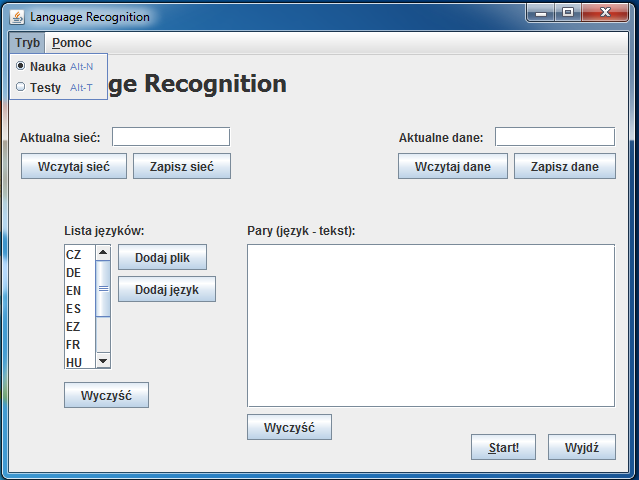
\includegraphics[width=3in]{GUI}
\caption{GUI. Widok ogólny}
\label{fig:gui}
\end{figure}

\begin{figure}[!t]
\centering
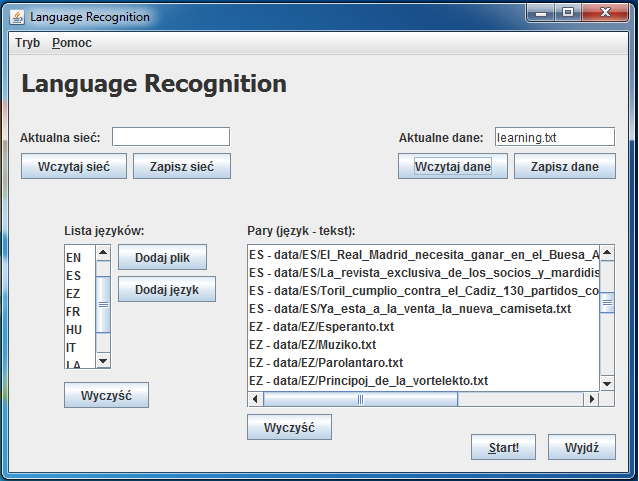
\includegraphics[width=3in]{Learning_ON}
\caption{GUI. Widok po załadowaniu zestawu danych}
\label{fig:gui_zestaw}
\end{figure}

Składa się z 5 głównych obszarów:
\begin{itemize}
 \item rozwijane menu wyboru trybu (Nauka/Testy),
 \item wczytywanie / zapisywanie pliku sieci neuronowej; podczas zapisu nie jest zapamiętywana lista obsługiwanych języków
- podczas wczytywania sieci należy zadbać o to, aby lista języków była taka sama jak podczas uczenia - w przeciwnym wypadku
test sieci może zwracać błędne wyniki,
 \item wczytywanie / zapisywanie pliku zestawu danych; po załadowaniu lista plików i ich języków pojawia się w polu
poniżej~(rys.~\ref{fig:gui_zestaw}),
 \item lista języków (możliwość dodania kolejnego / wyczyszczenia listy),
 \item lista aktualnie załadowanych plików i ich języków (możliwość dodania kolejnego / wyczyszczenia listy); aby dodać
kolejny plik należy wpierw zaznaczyć odpowiedni język na liście, a następnie wybrać opcję Dodaj plik.
\end{itemize}

\begin{figure}[!t]
\centering
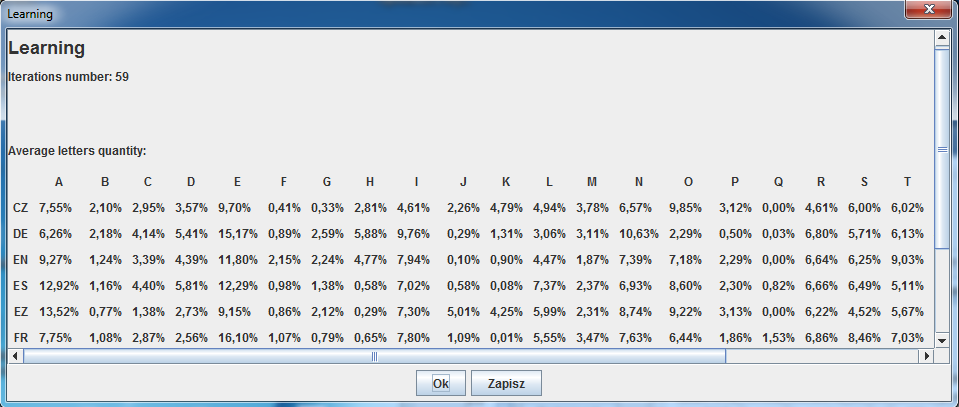
\includegraphics[width=3in]{Learning}
\caption{Okienko z wynikami. Uczenie}
\label{fig:learning}
\end{figure}

\begin{figure}[!t]
\centering
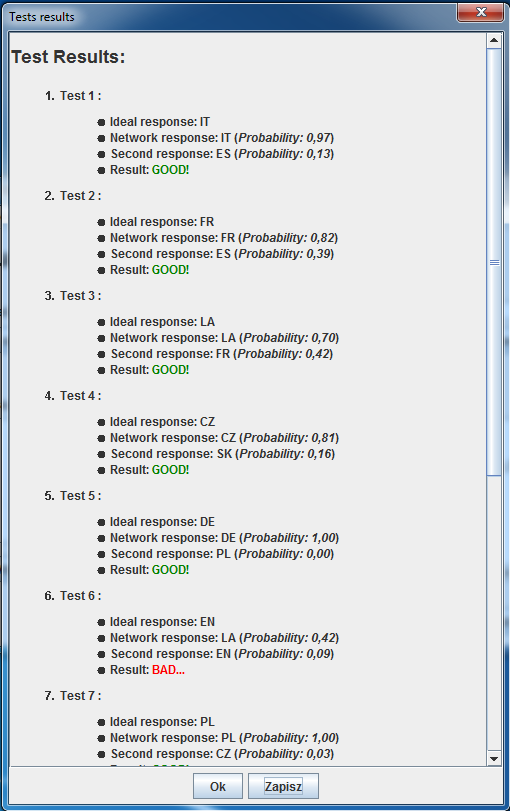
\includegraphics[width=3in]{Testing}
\caption{Okienko z wynikami. Testowanie}
\label{fig:testing}
\end{figure}

\begin{figure}[!t]
\centering
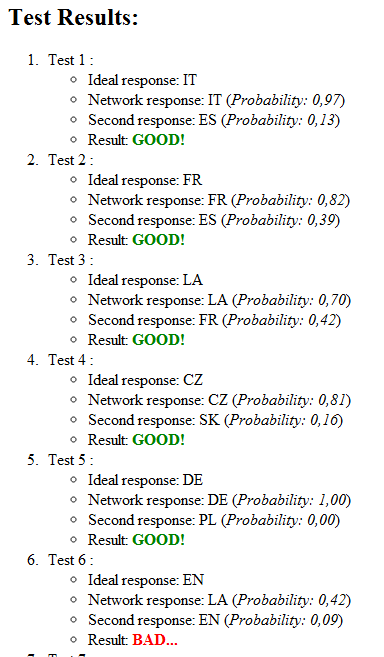
\includegraphics[width=2.7in]{TestResults}
\caption{Plik TestResult.html}
\label{fig:testing_file}
\end{figure}

Po zakończeniu procesu uczenia / testowania sieci, pojawia się okienko z wynikami:
\begin{itemize}
 \item uczenie: informacja o ilości iteracji oraz tabela ze średnimi częstotliwościami liter dla każdego języka
w zadanym zestawie uczącym~(rys.~\ref{fig:learning}),
 \item testowanie: informacja o każdym przeprowadzonym teście: prawidłowa odpowiedź, dwie najbardziej prawdopodobne odpowiedzi
udzielone przez sieć oraz ich prawdopodobieństwo, informacja o wyniku testu (GOOD / BAD); na końcu wyświetlana jest informacja
o obliczonej skuteczności sieci~(rys.~\ref{fig:testing}).
\end{itemize}
Istnieje możliwość zapisania raportu z wynikami do pliku html, odpowiednio LearnInfo.html
i~TestResult.html~(rys.~\ref{fig:testing_file}).


\section{Testy}
\IEEEPARstart{C}{elem} przetestowania aplikacji, przygotowano zestaw 5 tekstów w 11 językach: 
czeskim (CZ), niemieckim (DE), angielskim (EN), hiszpańskim (ES), esperanto (EZ), francuskim (FR),
węgierskim (HU), włoskim (IT), łacinie (LA), polskim (PL) i słowackim (SK). Dla każdego z języków 4 teksty posłużyły
do nauki, a piąty do testowania (nieobecny w zbiorze uczącym).

Osiągnięto skuteczność sieci na poziomie 90\% (średnio 1~błąd w zestawie 11 testów).

W poszczególnych testach osiągano różną pewność odpowiedzi sieci. Jest to ściśle zależne od tego, czy w zestawie występuje język
o podobnej częstotliwości liter. Przykładowo:
\begin{itemize}
 \item języki niemiecki i polski były rozpoznawane z pewnością na poziomie 95-100%,
 \item łacina i wywodzące się z niej języki romańskie: hiszpański, włoski, francuski były rozpoznawane z dużo mniejszą
skutecznością (30-70\%),
 \item języki czeski i słowacki, uważane za podobne do siebie, były zdecydowanie rozróżniane:
  \begin{itemize}
   \item test czeski: sieć odpowiedziała, że na 81\% jest to język czeski, natomiast język słowacki tylko na 16\%;
   \item test słowacki: sieć odpowiedziała, że na 90\% jest to język słowacki, natomiast język czeski tylko na 1\%.
  \end{itemize}
\end{itemize}

Skuteczność sieci zależy również ściśle od zbioru danych uczących. Powinno się w nim znajdować jak najwięcej tekstów,
odpowiedniej długości (im dłuższe tym lepsze). W~wykorzystanym zbiorze pojawiały się np teksty piosenek składające się tylko
z kilku zwrotek, co mogło okazać się zbyt krótką próbką języka i mogło utrudniać naukę sieci.

Na skuteczność sieci może wpływać również liczba neuronów w warstwie ukrytej, o czym już wcześniej wspomniano. W trakcie
testów wypróbowano kilka różnych wartości, jednak nie osiągnięto istotnych różnic. Zdecydowano się pozostawić 10 neuronów
w~tej warstwie.


\section{Wnioski}
\IEEEPARstart{Z}{} programistycznego punktu widzenia aplikacja była prosta i implementacja nie stwarzała większych
problemów, wymagała przede wszystkim odpowiedniej ilości poświęconego czasu.

Rozważany problem okazał się bardzo ciekawym od strony poznawczej. Zmierzenie się z zadaniem pozwoliło zapoznać się
z~dostępnymi materiałami na temat technik rozpoznawania języka tekstu. Testowanie większej ilości języków, niż początkowo
zakładane trzy, pozwoliło na odkrycie wiedzy, której autorzy wcześniej nie posiadali (m.in. o dużej różnicy pomiędzy
językami czeskim i słowackim).

Wyświetlenie tabeli z informacjami o częstotliwości występowania liter w poszczególnych językach pozwoliło na prowadzenie
własnych poszukiwań podobieństw i różnic między językami. W ramach rozwoju projektu warto zwizualizować sieć i przedstawić
wagi, które są ustalane w procesie uczenia - może to pozwolić na zobaczenie zależności, których nie widać ``na pierwszy
rzut oka''.

Projekt można również rozwinąć o stosowanie innych technik rozpoznawania języka, np obsługiwać wszystkie dostępne znaki
danego alfabetu, a nie tylko litery alfabetu łacińskiego, jak to zrobiono w niniejszym projekcie.

Walory poznawcze z pewnością będzie posiadało rozszerzenie projektu o obsługę kolejnych języków i zwiększenie ilości plików
w zbiorze uczącym. Stworzona aplikacja pozwala na dowolne rozszerzanie tych dwóch zbiorów, co zachęca do dalszych
eksperymentów.


% if have a single appendix:
%\appendix[Proof of the Zonklar Equations]
% or
%\appendix  % for no appendix heading
% do not use \section anymore after \appendix, only \section*
% is possibly needed

% use appendices with more than one appendix
% then use \section to start each appendix
% you must declare a \section before using any
% \subsection or using \label (\appendices by itself
% starts a section numbered zero.)
%


% Can use something like this to put references on a page
% by themselves when using endfloat and the captionsoff option.
\ifCLASSOPTIONcaptionsoff
  \newpage
\fi


% trigger a \newpage just before the given reference
% number - used to balance the columns on the last page
% adjust value as needed - may need to be readjusted if
% the document is modified later
%\IEEEtriggeratref{8}
% The "triggered" command can be changed if desired:
%\IEEEtriggercmd{\enlargethispage{-5in}}

% references section

% can use a bibliography generated by BibTeX as a .bbl file
% BibTeX documentation can be easily obtained at:
% http://www.ctan.org/tex-archive/biblio/bibtex/contrib/doc/
% The IEEEtran BibTeX style support page is at:
% http://www.michaelshell.org/tex/ieeetran/bibtex/
%\bibliographystyle{IEEEtran}
% argument is your BibTeX string definitions and bibliography database(s)
%\bibliography{IEEEabrv,../bib/paper}
%
% <OR> manually copy in the resultant .bbl file
% set second argument of \begin to the number of references
% (used to reserve space for the reference number labels box)
\begin{thebibliography}{1}

\bibitem{smykowski:jak_google_rozpoznaje}
T.~Smykowski, \emph{Jak Google rozpoznaje język tekstu?},
http://polishwords.com.pl/blog/2009/rozpoznawanie-jezyka-tekstu/,
(dostęp: 2012-05-31)

\bibitem{tad:elem_wpr}
R.~Tadeusiewicz, \emph{Elementarne wprowadzenie do techniki sieci neuronowych
z przykładowymi programami}, Warszawa, Polska: Akademicka Oficyna Wydawnicza PLJ, 1998.

\bibitem{tad:sieci}
R.~Tadeusiewicz, \emph{Sieci neuronowe}, wyd.~2, Warszawa, Polska: Akademicka
Oficyna Wydawnicza RM, 1993.

\bibitem{ethnologue}
\emph{Ethnologue}, http://www.ethnologue.com/language\_index.asp,
(dostęp: 2012-05-31)

\bibitem{wiki:langs}
\emph{Language recognition chart}, \\ http://en.wikipedia.org/wiki/Wikipedia:Language\_recognition\_chart,
(dostęp: 2012-05-31)

\bibitem{encog:rprop}
\emph{Resilient Propagation}, \\ http://www.heatonresearch.com/wiki/Resilient\_Propagation,
(dostęp: 2012-05-31)

\bibitem{wiki:scrabble}
\emph{Scrabble letter distributions}, \\ http://en.wikipedia.org/wiki/Scrabble\_letter\_distributions,
(dostęp: 2012-05-31)

\bibitem{wiki:sieci}
\emph{Sieć neuronowa}, http://pl.wikipedia.org/wiki/Sieć\_neuronowa,
(dostęp: 2012-05-31)


\end{thebibliography}

\end{document}

